\documentclass{report}
\usepackage[utf8]{inputenc}
\usepackage[danish]{babel}
\usepackage{amsmath}
\usepackage{graphicx}
\usepackage{subfig}
\begin{document}
\setcounter{chapter}{0}

%Forside
\title{Projektarbejde, Snake}
\date{18. januar, 2015}
\author{	Anna Ølgaard Nielsen - 			s144437\\
Christian Søholm Andersen 	- s103080\\
Mathias Enggrob Boon - 			s144484\\
Van Anh Tri Trinh - 				s144449}

\maketitle

%Indholdfortegnelse
\tableofcontents
\newpage
\setcounter{chapter}{0}
%Første side
\pagenumbering{arabic}
\chapter{Introduktion}
Formålet med projektopgaven er at genskabe det klassiske spil \textbf{Snake}, samt at dokumentere hvordan spillet er lavet.
Spillet er gengivet i to versioner: \textbf{Simpel Snake} og \textbf{Avanceret Snake}. Simpel Snake er en primitiv version af spillet, hvor styring og bevægelse kun foregår vha. input fra spilleren. I Avanceret Snake er der tilføjet forskellige funktioner, som enten forbedrer brugerfladen - f.eks. tilføjelse af hovedmenu - eller ændrer spillet - f.eks. automatisk bevægelse af slangen.
I rapporten vil designet af begge spillets versioner blive forklaret, samt implementationen af spillet. Kapitlet "Udviklingsproces" forklarer de tanker, der ligger bag implementationen, og de valg der er foretaget, når der er flere mulige implementationer.

\begin{figure}[b]
	\centering
	\graphicspath{ {pics/} }
	\subfloat[Simpel Snake]{\label{fig:simplesnake}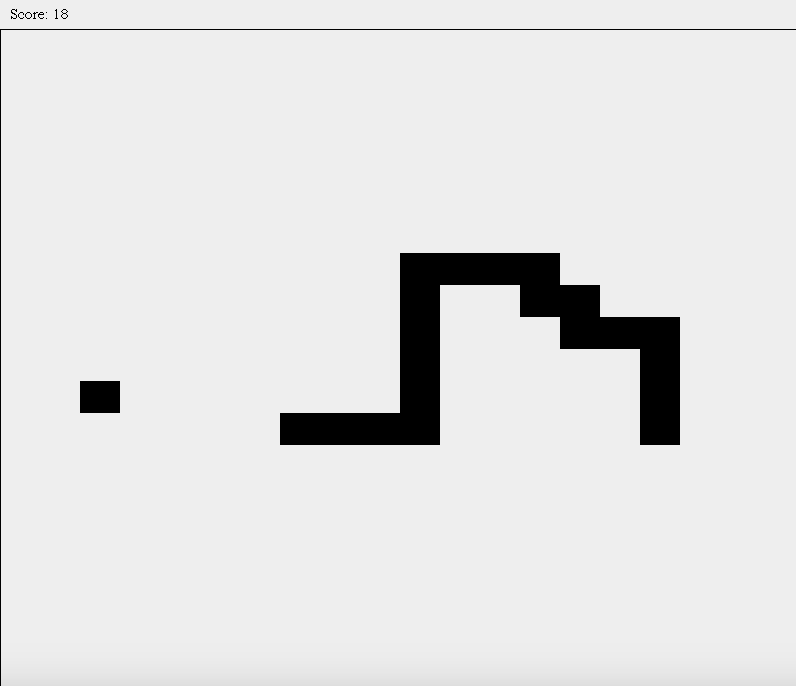
\includegraphics[width=0.4\textwidth]{SimpelSnake.png}}
	\hspace{0.1\textwidth}
	\subfloat[Advanced Snake]{\label{fig:advancedsnake}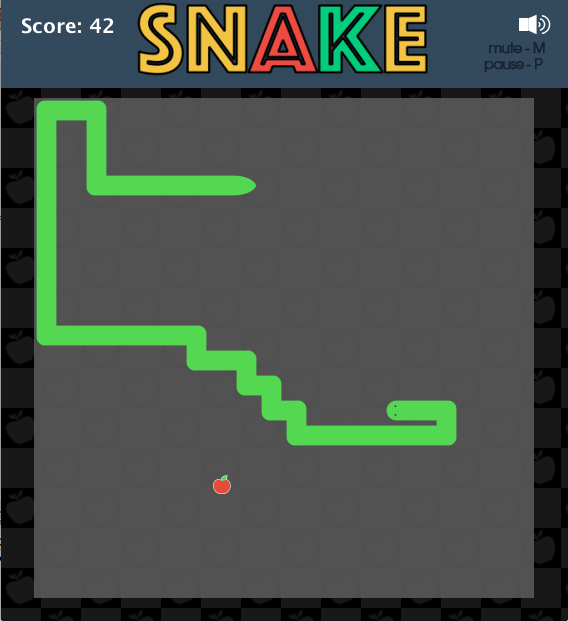
\includegraphics[width=0.32\textwidth]{snake2.png}}
\end{figure}

\chapter{Simpel Snake}
\section{Afgrænsning}
I Simpel Snake består slangen af to felter (et hoved og en hale), der er placeret banens centrum med retning mod venstre. Det er muligt gennem input fra tastaturet at bevæge sig frit på banen i de fire retninger i et almindeligt koordinatsytem: op og ned ad y-aksen og hen ad x-aksen i begge retninger - dog ikke modsatrettet slangens bevægelsesretning. Bevæger man sig ud over banens kanter, skal man kunne fortsætte på den modsatte side. Det skal derudover være muligt at øge slangens længde ved at bevæge sig over et felt med et "æble". Spillet slutter, når spilleren har fyldt hele banen ud med slangens krop og dermed har vundet spillet, eller ved at spilleren bevæger sig ind i et felt udfyldt af slangen, der ikke er halestykket, som ved slangens bevægelse også rykker videre til et nyt felt. I så fald, har spilleren tabt spillet.
\linebreak

\section{Design}
Simpel Snake er designet, så selve spillets funktioner ligger i klassen \textit{Game} i model-pakken. \textit{Game} får da spillets objekter fra andre klasser i \textit{model}-pakken, f.eks. Board (spillebrættet) og Snake (slangen). Spillets tilstand ændres, når der modtages input fra \textit{control}-klasserne, som bestemmer hvornår og hvordan slangen bevæger sig. I \textit{??}-klassen er en observer, som notificeres hver gang banens tilstand ændres. Når dette sker, eller når spillet startes, tegnes banen vha. klasserne \textit{View} og {BoardPanel}. Disse klasser modtager information fra \textit{model}-klasserne, f.eks. \textit{Snake}, til at bestemme hvordan spillet gentegnes. \textit{BoardPanel} gentegner hele spillet hver gang spillet opdateres. Først tegnes selve banen, derefter slangen og til sidst æblet. 
For at starte spillet bruges klassen \textit{Driver}, som opretter et nyt \textit{Game}-, \textit{View} og \textit{Control}-objekt.
\linebreak

Snake-spillet er lavet efter et \textit{Model-View-Controller}-design (MVC), hvorved selve spillet, styringen af spillet og den visuelle repræsentation af spillet holdes adskilt i tre dele. På denne måde interagerer brugeren kun med den del af programmet, der er dedikeret til styring. Styringen manipulerer programmets tilstand i \textit{model}-koden, som visualiseres i \textit{view}-koden. Dette betyder derfor også, at alle funktioner, der påvirker programmets tilstand, skal holdes i \textit{model}-koden. \textit{Control} modtager kun input fra brugeren, og sender dette videre til \textit{View} og/eller \textit{Model}. \textit{View} modtager input fra \textit{Control} og sender ændringerne i \textit{View} videre til \textit{Model}. Det er derefter muligt gennem en observer at "observere" ændringerne i \textit{Game}, som bliver opdateret i \textit{View}.

\section{Implementering}

\subsection{Model}
Spillets model består af en række klasser, der tilsammen udgør selve spillets funktioner og objekter.
Klassen \textit{Field} bruges til at definere et objekt, som opdeler banen og repræsenterer et felt i banen. Den fungerer på samme måde som \textit{Point}-objekt-klassen, hvor koordinatsystemet starter oppe i venstre hjørne. Den eneste forskel mellem \textit{Point}- og \textit{Field}-klassen, er hvordan man kommer frem til et punkt. \textit{Point}-klassen går først ud ad x-aksen og derefter ned ad y-aksen, hvorimod \textit{Field}-klassen gør det i omvendt rækkefølge. Da hele vores spilleplade er delt op i rows og column frem for x og y, er \textit{Field} lettere at bruge for at undgå forvirring (????).
\linebreak

Funktionenen \textit{equals} er defineret i denne klasse, og bruges til at undersøge om to objekter ligger på samme felt, f.eks. slangens hoved og æblet. Æblet er defineret i klassen \textit{Food}, hvor datafeltet \textit{position} afgør dets nuværende position. 

Slangen selv er defineret i klassen \textit{Snake}. Slangens krop består af en række felter, hvoraf det første er hovedet, og de resterende er kroppen. Koordinaterne for disse felter er gemt som elementer i en LinkedList (???) kaldet \textit{positions}. Det første element er slangens første led, hovedet, andet element er slangens andet led osv. Når et nyt led tilføjes, tilføjes et nyt element til listen. Dette bruges, når slangen spiser et æble. Her ligger slangen stille, mens et nyt hoved tilføjes i æblets felt i den retning, der er trykket. 
((((Vi bruger linkedlist i stedet for arraylist, som vi startede med, fordi når man hver gang tilføjer et nyt hovede, så får hovedet den første plads, og alle andre elementer flyttes en gang tilbage. Når slangen er stor nok, kan dette godt komme til at lacke spillet lidt. Derfor er linkedlist helt klart mest optimalt at bruge, da den bare tilføjer et nyt element forrest uden at rykke alle de andre elementer.)))) - evaluering?

Funktionen \textit{setupStartingSnake} opretter en slange ved at beregne banens centrum, og tilføje to elementer til \textit{positions}-listen: centrumfeltet og feltet til højre for dette felt.

Selve banen er defineret i \textit{Board}-klassen, som har datafelterne \textit{height} og \textit{width}. Funktionen \textit{wrap} undersøger om slangen er ved at bevæge sig ud over banens grænser. Er dette tilfældet, fortsætter slangen i stedet på den modsatte side af banen.

Når \textit{move}-funktionen kaldes, undersøges der først, om den nye retning er modsatrettet slangens nuværende retning. Er dette tilfældet, sker intet. Er retningen gyldig, undersøges der om der ligger et æble på den nye plads. Hvis der gør, tilføjes et nyt element i ArrayListen \textit{positions}.
Der undersøges næst, om slangen rammer sig selv, ved at sammenligne om det ønskede felt har samme koordinater som et af slangens led, udover halen. Er dette tilfældet, sættes spillets tilstand til \textit{LOST}, hvorved spillet slutter. Hvis ikke, flytter slangen sin position, således at hovedet indtager et nyt felt, andet led tager hovedets tidligere plads, tredje led tager andet leds plads osv. Dette gøres ved, at ArrayListen opdateres bagfra, således at halen tager næstsidste leds koordinater, næstsidste led tager tredjesidste led osv. Når dette er gjort, tager hovedet den nye position, som afhænger af hvilket input der gives.

For at sikre, at maden altid placeres på et gyldigt felt, benyttes funktionen generateRandomFood i Food-klassen. Så længe slangen er under en hvis størrelse, placeres maden på et tilfældigt felt, hvorefter det sikres at feltet ikke er optaget af slangen. Er den det, placeres maden et nyt sted.

Er slangen større end $2*bredde*højde$, laves en ArrayListe over de felter, maden kan placeres på, hvorefter maden placeres tilfældigt på en af disse felter.

\subsection{View (Brugergrænseflade)}
Brugerfladen er samlet i klassen \textit{View} der [EXTENDS] \textit{JFrame}. I \textit{View} oprettes et score-panel, der placeres øverst i vinduet, og et board-panel, der placeres lige under det. Board-panelet viser selve spillepladen med slangen og æblet, der begge er vist ved farvede firkanter, som repræsenterer felterne i brættet, hvor slangen og æblet ligger.

\subsection{Control (Styring)}
I Simpel Snake bruges kun fire taster til input, nemlig de fire piletaster, som derfor er defineret i \textit{Control}.\textit{Control}-klassen har metoden, \textit{keyPressed}, som kaldes hver gang der tastes på tastaturet. Hvis tasten er en af de fire piletaster, kaldes funktionen \textit{moveSnake} i \textit{Snake}-klassen, med den tilsvarende retning som parameter.

\section{Udviklingsproces}
\subsection{Arbejdsproces}
Formålet med projektet var at starte med at lave en simpel udgave af snake, og derefter tilføje flere funktioner til at lave en mere avanceret version. Dette gør det ideelt at tilføje en funktion af gangen, hvormed programmet starter ud simpelt, men fungerende, hvorefter yderligere funktioner kan tilføjes. Programmet er altså udviklet iterativt, hvorved der opstår flere fungerende versioner af spillet, men med forskellige funktioner. Dette gør det muligt at tilpasse programmet, hvis der opstår nye idéer undervejs. 

Den iterative tilgang gør det muligt at have en "cyklus" for udviklingen af programmet. Først bestemmes det, der skal tilføjes til programmet. Derefter fordeles opgaverne blandt gruppens medlemmer. Gruppemedlemmet afgør selv, hvordan en funktion skal designes og implementeres. Når en ny tilføjelse til programmet er færdig, testes den. Eventuelle justeringer til programmet laves for at undgå fejl med den nye funktion, hvorefter "cyklussen" starter forfra ved

\subsection{Controller}
	
\subsection{Model}

\subsubsection{Opbygning af banen}
Til designet af selve banen, som slangen bevæger sig på, forelås to muligheder. Den ene er at lave et to-dimensionelt array af datatypen enum, hvis størrelse afgør banens endelige størrelse. Et array [10][5] vil f.eks. give en bane med længden 10 og bredden 5. Hvert element i arrayet bestemmer da, hvad der befiner sig på netop denne plads på banen. Elementerne i arrayet kan f.eks. være et blankt felt, et æble, et led af slangen osv. Dette gør det nemt at introducere nye spilelementer i fremtiden, f.eks. bonus-point, vægge og miner, idet der blot skal tilføjes nye værdityper. Visualisering af spillet foregår ved at definere et billede for hvert spilelement, og få programmet til at tegne objektet på arrayets plads.
ULEMPER - observer?

En anden metode er, at lade de forskellige spilelementer være defineret i deres egne klasser, så f.eks. er \textit{SnakeFood} en klasse for sig selv, \textit{SnakePlayer} er en klasse for sig selv osv. Hver klasse har de funktioner, der er relevante for dem, f.eks. \textit{getPosition} for at give deres nuværende position. Programmet tegner da spillet hver gang en tur afsluttes, dvs. når alle elementer som skal ændres, er ændret. Programmet har fået defineret billedet for de forskellige elementer, og modtager deres position vha. en \textit{getPosition} metode.
 Ulempen ved denne metode er, at tegning af programmet gøres mere kompliceret. I den første metode er alle felter allerede defineret, og for at ændre dem behøves der blot at ændre værdien. Ønskes et spilelement ændret eller introduceret med den anden metode, skal der laves et nyt objekt.
 
Den anden metode blev valgt til spillet, idet det blev bestemt at den passede bedre til MVC-modellen, idet view-koden kun bruger de forskellige klassers \textit{get}-metoder til at få information. %bum bum

\subsubsection{Snake}
Da slangen i snake-spillet består af en række felter, som alle har netop et koordinat i forbindelse med de resterende, er en effektiv måde at bestemme slangens position på en LinkedList, idet denne datastrukturer er fleksibel i størrelse og passer til formålet. Når slangen vokser i størrelse, bliver dette dog mindre effektivt, idet slangens hoved altid er element 0. Når slangen vokser, tilføjes et nyt element på plads 0, hvormed hele listen skal flyttes. En anden mulighed ville være at bruge en anden datastruktur, f.eks. LinkedList, eller lade hovedet være defineret som element positions.size()-1, hvormed nye hovedet tilføjes sidst i listen.

For at implementere scoren blev der fremlagt to løsninger. Enten at lade scoren være et datafelt i game-klassen, eller at lade det være en klasse for sig selv. Ved at lade scoren være et datafelt, bliver implementationen simplere. At lade scoren være en klasse for sig selv har derimod fordelen, at der kan 
tilføjes en observer til Score-klassen, som dermed kun opdateres, når scoren ændrer sig. Scorepanelet tegnes ikke i samme klasse som banen, og kan derfor holdes seperat, så scorepanelet kun gentegnes, når scoren ændrer sig. Hvis scoren derimod er et datafelt, tegnes scoren efter hver tur, også selvom scoren er uændret. I sidste ende blev det bestemt at holde scoren som datafelt, hvormed det også bliver simplere at implementere nye score-relaterede funktioner i fremtidige udgaver.

\subsection{Brugergrænseflade og visualisering af programmet}
\subsubsection{Tegning af banen}


\subsubsection{Vinduesstørrelse}
Området, som spillet foregår på, skal kunne bestemmes til at være mellem 5x5 og 100x100. Dette kan dog skabe problemer, hvis størrelsen bliver for stor, idet banen både skal være synlig, men også passe på en gennemsnitlig computerskærm. En bane på 10x10 kan sagtens passe på en opløsning af f.eks. 400x400, men øges banens størrelse til 50x50, bliver banen svær at se. Herudover varierer skærmstørrelser, og det er derfor nødvendigt at gøre spillets vinduestørrelse fleksibel. En løsning på dette problem ville være at bestemme en fast størrelse for felterne, og lade vinduet justere sin størrelse efter dette. Ønskes det f.eks. at felterne altid har størrelsen 20x20, og at banen skal være 15x25, vil vinduets størrelse blive 300x500. Fordelen ved denne metode er at det sikres, at banen altid er synlig, og at der ikke opstår problemer, fordi forholdet mellem vinduets størrelse og banen størrelse ikke passer sammen. Ulempen ved metoden er, at store baner kan blive for store til at være på en normal skærm. F.eks. vil en bane med felter af størrelsen 20x20 og banestørrelsen 75x75 fylde 1500x1500. Herudover er løsningen ikke brugervenlig, idet en bruger kan blive forvirret over hvorfor vinduets størrelse ændrer sig fra bane til bane, og måske ligefrem ikke passer på skærmen.

En anden metode er at gøre vinduet justerbart. Denne løsning er mere brugervenlig, idet vinduets størrelse frit kan justeres så det passer til den enkelte person. Denne metode introducerer dog et andet problem, nemlig at felternes størrelse skal skaleres til at passe vinduet. Nogle opløsninger af vinduet vil ikke være et multiplum af banens størrelse, hvormed elementerne i spillet vil blive aflange. Dette problem blev løst ved at lave en baggrund og låse banens forhold, hvormed banen altid fylder mest muligt af vinduet ud, og den resterende plads bliver udfyldt af baggrunden. Idet denne løsning var nemmere at bruge og forstå, og giver bedre mulighed for justering af spillet, blev den valgt i stedet for den første løsning.
\begin{figure}[h]
	\centering
	\graphicspath{ {pics/} }
	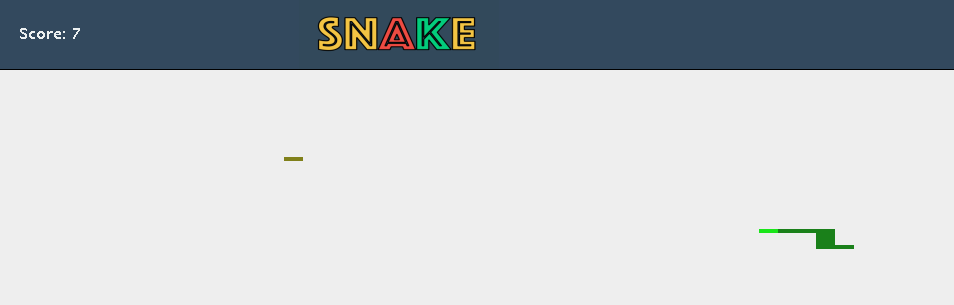
\includegraphics[width=0.5\textwidth]{WindowSize.png}
	\label{fig:windowsize}
	\caption{windowsize}
\end{figure}


\section{Evaluering}
-To eller en Arraylist -> linklist ?
-Point -> Field
-Int -> Enum (direction)
-width+height <-> kvadratisk variabel ?
-Banens opbygning: double-array -> positions-placering
-Optimering af runtime i “food”-klassen (dobbelt for-loop eller random placering)
-brug af observer - får model-view-controller til at gå op
-Flere opgaver er givet til “game”-klassen frem for de andre klasser

\chapter{Avanceret Snake}
\section{Afgrænsning}
I den avancerede del af spillet skal slangen bevæge sig ved hjælp af en timer og altså ikke vente på input fra tastaturet. Input fra tastaturet ændrer derimod kun retning eller sætter farten op. Derudover skal slangen accelerere - dvs. slangens hastighed øges efter et vis antal samlede æbler, hvilket gør spillet mere udfordrende og mindre ensartet. Vi har derudover også valgt at lave spillet, som skulle det udgives helt færdiggjort. Derfor er det holdt simpelt med kun få funktioner. Der er derimod lagt fokus på høj kvalitet af spillets grafik og brugervenlighed med hensyn til navigering. Brugergrænsefladen skal tilpasses brugerens skærmstørrelse, ønskede vinduesstørelse og brugerens operativsystem. Det skal også være muligt at navigere både igennem tastatur-input og mussekliks-input. Brugeren skal derudover også have frihed til at vælge slangens hastighed og farve og banens størrelse - stadig uden at dette kommer til at hæmme spillets udseende eller kvalitet. Simpel Snakes bevægelsesfunktion, der ikke er afhængig af en timer, er beholdt som en "kindergarten"-sværhedsgrad, som brugeren kan vælge i menuen.

-----Skriv om multiplayer + evt. netværk---------


\section{Design}
I \textit{Driver}-klassen, der får spillet til at køre, oprettes tre objekter fra de tre hovedklasser \textit{Game}, \textit{View} og \textit{Control}, der hver især står for henholdsvis \textit{Model}, \textit{View} og \textit{Control} i \textit{Model-View-Controller}-designet.

I JFrame'n \textit{View} oprettes spillets scener repræsenteret af andre view-klasser i samme pakke. Disse view-klasser er alle JPanels som tilføjes til vinduet og skiftes ud alt efter hvor i spillet spilleren befinder sig, i hovedmenuen, i singleplayer-menuen, i selve spil-scenen, osv. På denne måde har hver scene i spillet en tilhørende klasse der [extends] JPaneler. Klasserne oprettes alle med View som parameter, og kan derfor give og bruge hinandens funktioner, idet View-klassen har getter-metoder til alle de andre view-klasser. View-klasserne kan derfor genbruge nødvendige metoder, f.eks. metoden til at tegne baggrunden op, der f.eks. skal være ens i alle paneler. Spilleren navigerer vha. JButtons eller tastatur-input der modtages i Control-klasserne.

Control-klassen er tilknyttet View, og virker derfor alle steder i spillet. Denne har funktioner såsom "mute" og "return to menu", som skal være fungerende uanset hvor i spillet spilleren er - altså hvilke paneler der er vist. I samme pakke ligger andre control-klasser, som alle hører til en bestemt scene. Dette sørger for at kontrolfunktionerne er unikke og kun fungerer på deres bestemte måder, hvis man er inde i deres bestemte scene.

I \textit{Model}-pakken findes den abstrakte klasse \textit{Game}, som klasserne \textit{GameSingleplayer} og \textit{GameMultiplayer} implementerer. [............]


\section{Implementering}

\subsection{Model}

\subsection{View (Brugergrænseflade)}
Al grafik, som ikke er fra \textit{Swing}-biblioteket, er importeret i en fælles klasse \textit{Image}, der gør det muligt for enhver view-klasse at få fat i alle billeder. På samme måde er selv-definerede farver oprettet i klassen Colors.
Når \textit{View}-klassen konstrueres opretter den i forvejen alle andre paneler, men tilføjer først \textit{ViewHeader}-panelet og \textit{ViewMenu}-panelet. Disse skiftes kun ud med andre paneler gennem input fra spilleren, når spilleren bevæger sig rundt i spillet. Denne frame bruger \textit{BorderLayout}, der gør det simpelt at placere \textit{ViewHeader}-panelet øverst, og det ønskede scene-panel nedenunder. Alle andre view-klasser er efterladt med standard-layoutet \textit{FlowLayout}, da deres komponenter skal placeres i specifikke koordinater. Dette gøres med \textit{setBounds} der definerer komponentets størrelse og placering. For at komponenterne følger med, når spilleren ændrer vinduets størrelse, er deres koordinater dog ikke altid bevaret hvis komponenterne f.eks. altid skal ligge i midten af vinduet. Disse kald på \textit{setBounds}-metoden er placeret i panelernes \textit{paintComponent}-metode da, denne køres hver gang vinduet skaleres. Koordinaterne beregnes derved påny hver gang vinduet skaleres, og komponenterne kan derfor altid få de rigtige koordinater. Denne metode er brugt til alle billeder, komponenter og tekst der oprettes eller tegnes.

\textit{ViewMenu} indeholder metoder der tegner flise-baggrunden og et gennemsigtigt område med scenens indhold. Disse metoder bruges også af alle andre paneler, da den samme baggrund skal tegnes. Som den eneste klasse opretter \textit{ViewMenuSingleplayer} sit eget panel der svarer til det gennemsigtige område, hvilket gør det lettere at beregne koordinaterne til alle panelets komponenter lettere, idet der ikke længere skal tages hensyn til flise-baggrunden, som også hører med til det oprindelige panel.

I klassen \textit{ViewBoard} tegnes grafikken til spillet. Her er lagt specielt vægt på, at felternes størrelse passer til spillerens ønskede bane-størrelse og spillerens ønskede vinduesstørrelse samtidig med at bevare deres kvadrate form. Metoden \textit{getFieldSideLength} beregner ud fra disse to størrelser den størst mulige længde og højde af et enkelt felt og returnerer derefter den mindste af de to værdier. På denne måde kan feltet være kvadratisk og passer med sikkerhed på begge led af vinduet. Denne \textit{getFieldSideLength}-metode kan nu bruges til at bestemme størrelsen af og tegne banen, slangen og æblet, så de passer til vinduets størrelse. Da disse tegnemetoder bliver kaldt fra \textit{paintComponent}-metoden, der køres igennem konstant under spillet og når vinduesstørelsen ændres, har spillets komponenter altid en passende størrelse.
Når spilleren færdiggør spillet enten ved at tabe eller vinde, tegnes \textit{Game Over}-skærmen ved en gennemsigtig rektangel, med \textit{Final Score} og JButtons, der giver mulighed for at gå tilbage til menuen eller spille igen.
Udover bane-størrelse er det også muligt at vælge slangens farve. Dette gøres lige før spillets start, når spilleren har valgt farve. Biillederne for slangen farves og kan derefter bruges til at tegne slangen. Slangen farves ved at køre hver enkel af et billedes pixel igennem og derefter give det en anden farve defineret ved tre heltal givet som parametre til \textit{colourSnake}-metoden, der farver den givne pixel, hvis dens farve ikke er svarende til slangens øjenfarve.

\subsection{Control (Styring)}
For at give spilleren valgfrihed er der til mange funktioner både implementeret en JButton og en tilhørende genvej gennem tastaturet. Fra tastaturet er der blevet implementeret følgende genveje: Mute-button (M), pause-button (P), menu-button (Esc), tilbage-button (Backspace), (re)start-button (enter/space), som (gen)starter spillet. \textit{Control}-klasserne [extends] \textit{KeyAdapter}, der registerer tastatur-input, og implementerer \textit{ActionListener}, der registrerer tryk på knapper. Disse klasser tilføjer \textit{KeyListeners} til \textit{View}-klassen, og \textit{ActionListener} til panelet, der indeholder den bestemme \textit{Control}-klasses knapper. Individuel kontrol over de forskellige knapper fås ved at sætte en unik \textit{ActionCommand} til hver enkel knap, der derefter kan tjekkes for i \textit{ActionListener}ens abstrakte metode \textit{actionPerformed}. Det er her også nødvendigt efter knappetryk at bruge \textit{requestFocus}-metoden på \textit{View}-klassen, da spillet efter knappetryk, får et nyt fokus, hvilket betyder, at tastatur-inputtet ikke opfattes af spillet.
Især når \textit{View} oprettes, bruges \textit{setFocusable}- og \textit{requestFocus}-metoden, eftersom tastatur-input allerede skal være brugbart her på grund af \textit{mute}-funktionen.
Før spillets start kan spilleren som tidligere nævnt - udover at vælge farve og sværhedsgrad - vælge banestørrelsen. Denne funktion er indbygget vha. to \textit{JFormattedTextFields} der har fået en \textit{Formatter}, som begrænser inputtet til højst et tre-cifret tal. Dette begrænser spillerens mulighed for at indtaste en ugyldig størrelse. Giver spilleren alligevel en ugyldig værdi (under 5 eller over 100) eller efterlader et felt tomt, printes en fejlmelding og spilleren kan ikke starte spillet før der er indtastet gyldige værdier. For alligevel ikke at gøre det svært for spilleren at indtaste rigtige værdier, ses der bort fra eventuelle mellemrum før, efter eller i midten af tallene, da disse fjernes før inputtet regnes om til et heltal, som derefter sammen med den valgte sværhedsgrad gives videre som informationer til \textit{model}-pakkens \textit{Game}-klasse. Farvevalget gives til \textit{view}-pakkens \textit{ViewBoard}-klasse, der farver billederne til slangen.

(((((((Da tekstfelterenes \textit{Formatter} får deres caret til at sætte sig i starten af tekstfeltet selvom spilleren trykker et andet sted i feltet, implementerer klassen en \textit{FocusListener}, der har de abstrakte metoder \textit{focusGained} og \textit{focusLost(...)}. I \textit{focusGained} oprettes )))))).

\section{Udviklingsproces}

\subsection{Tegning af slangen}
I Simpel Snake kan spilleren ud fra slangens krop se hvor han har været, men ikke hvilken vej han har bevæget sig, idet de udfyldte felter er fyldt helt ud til kanten[FIG HENVISNING]. Slangens udseende kan derfor forbedres ved at vise slangens bevægelsesretning og retningsskift i hver enkel del af dens krop og generelt erstatte alle firkanterne, med mere beskrivende billeder [FIG HENVISNING]. Dette giver seks mulige udseender for hver enkel del af slangen udover hovedet og enden af halen, der hver findes i fire versioner afhængig af retningen, som spilleren vælger for hovedet, eller retningen af kropsdelen lige før halen. Kropsstykkerne imellem er dog ikke kun afhængig af retningen af stykket lige før eller lige efter, men begge dele. Den vandrette del og den lodrette del af slangen bestemmes let ved at undersøge om stykket, der skal tegnes ligger i samme række eller kolonne som stykkerne før og efter. Slangens hjørnestykker bestemmes på en mere indviklet måde, da stykket og dens tilgrænsende stykker aldrig ligger i samme række eller kolonne, men derimod kan ligge i fire forskellige forhold til hinanden (Se figur 3.1). I figur \ref{fig:corner1} ligger de tilgrænsende felter lige under og til højre for hjørnet, men dette gælder f.eks. ikke for figur \ref{fig:corner3} hvor det ene stykke ligger lige under, mens det andet stykke ligger til venstre for hjørnet uden at grænse op til dens venstre side, der ellers ville give hjørnestykket spejlvendt i y-aksen. Da felterne ligger i en XXXXX-liste sorteret efter slangens opnåede dele, sammenlignes et felt med feltet før og efter det i listen. Da stykket foran og bagved uden påvirkning på hjørnestykket kan bytte plads, findes der altså otte situationer for et enkelt hjørnestykke. I alt tjekkes der derfor - for kroppen alene - 34 mulige forhold mellem et stykke og dens to tilgrænsende stykker.
\linebreak

I \textit{ViewBoard}-klassen er der lavet en \textit{drawSnake}-metode, der består af en del if-statements, for hvilket figur af slangen, der skal bruges i en bestemt retning. I \textit{snakeCorner}-metoden returnerer den en lang boolean \textit{isCorner}, som tidligere har været kopieret 4 gange for de fire retninger, men som nu er blevet simplificeret med en masse variable til den samme boolean. Måden det blev gjort på, var at finde et mønster i de fire lange booleans før og så indsætte 12 forskellige varibale, der gjorde det muligt kun at kalde en boolean. På samme tid kører programmet ikke alle if-else-statements igennem hver gang den skal lave et hjørne, men kun det hjørne som bliver kaldt. Variablerne kan enten have værdien 0, 1, -1, lastColumn eller lastRow. Da det specifikke hjørne skal dukke op et bestemt sted alt efter hvor på banen slangen befinder sig.
De første to rækker kode af \textit{isCorner}, fortæller om når slangen er placeret midt på banen (se figur \ref{fig:corner1}), og drejer til den specifikke retning, så må det foranliggende (front) og bagvedliggende stykke (behind) ligge et bestemt sted, som enten getColumn()+1 eller getColumn()-1 og på samme måde getRow()+1 eller getRow()-1. I de to næste ligner kode i \textit{isCorner} beskriver den, hvis slangen er placeret på den sidst række (altså i bunden af banen) og går gennem torussen, så den ender øverst i banen (se figur \ref{fig:corner2}).
De to næste linjer kode er på samme måde, når slangen ligger yderst til højre eller venstre og går gennem torussen (se figur \ref{fig:corner3}).
De to sidste linjer kode er til, når slangen går gennem torussen to steder i et af hjørnerne. Altså hvis slangen f.eks. er nede i højre hjørne, går gennem torussen ved at gå ned ad, og straks til højre gennem torussen igen (se figur \ref{fig:corner4}). 
Derved er alle hjørne-situationer gennemgået.
Man kan se et mere detaljeret billede af snake-kroppen i Appendix [INDSÆT HENVISNING].
\begin{figure}[h]
	\centering
	\graphicspath{ {pics/} }
	\caption{}
	\subfloat[Corner 1]{\label{fig:corner1}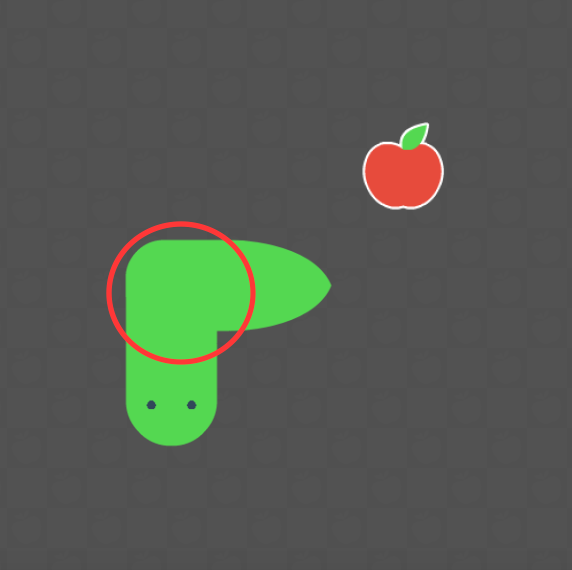
\includegraphics[width=0.15\textwidth]{Corner1.png}}
	\hspace{0.05\textwidth}
	\subfloat[Corner 2]{\label{fig:corner2}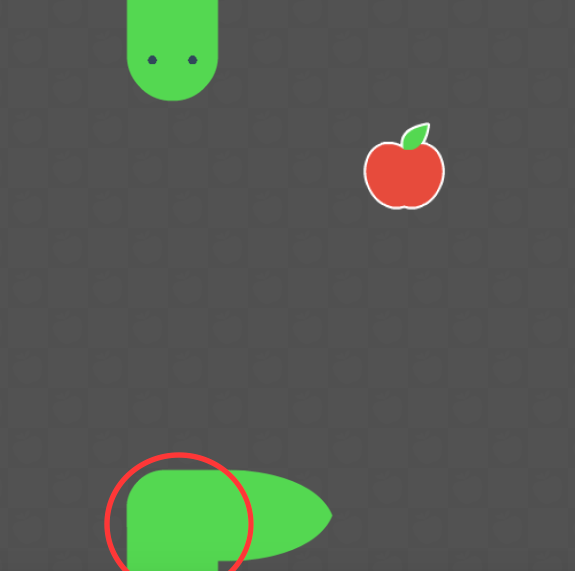
\includegraphics[width=0.15\textwidth]{Corner2.png}}
	\hspace{0.05\textwidth}
	\subfloat[Corner 3]{\label{fig:corner3}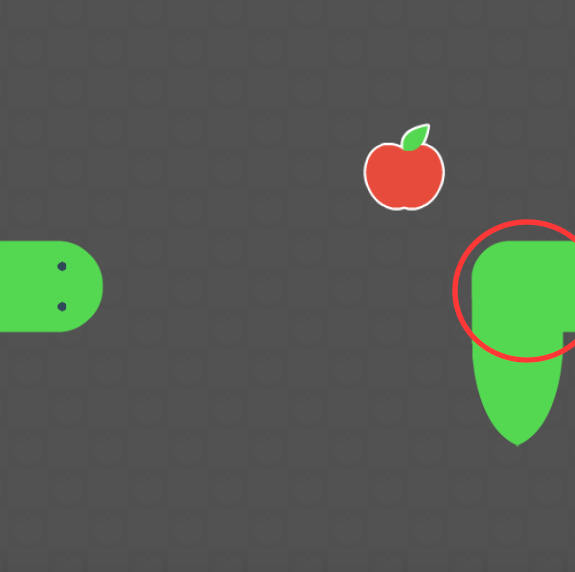
\includegraphics[width=0.15\textwidth]{Corner3.png}}
	\hspace{0.05\textwidth}
	\subfloat[Corner 4]{\label{fig:corner4}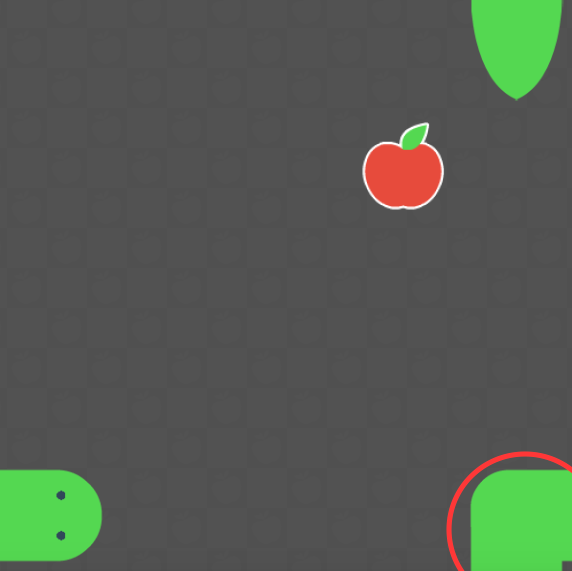
\includegraphics[width=0.15\textwidth]{Corner4.png}}
\end{figure}

\subsection{Lyd}

Som en mindre tilføjelse til spillet er lyd tilføjet i form af Audio-klassen. Funktionerne i Audio-klassen bruges til individuelt at spille 	


\subsection{Menu}

\subsection{Automatisk bevægelse}
-----Husk at skriv noget om incrementet timer-------

\subsection{Multiplayer}

\section{Evaluering}
For at sikre stabilitet af brugergrænsefladen er spillet afprøvet i forskellige størrelser og på forskellige operativsystemer. Placeringen af komponenterne er ens i Micrsoft Windows 8.1 og dens ældre versioner, [INSERT---------]. Derimod har JButtons et lidt andet udseende på [INSEEEEERT], idet deres baggrundsfarve i dette operativsystem ikke er synlig medmindre deres kant skjules. Derudover virker de her heller ikke, hvis de tilføjes til et panel i \textit{paintComponent}-metoden. Det første problem løses ved at skjule kanten eller i stedet at bruge et ImageIcon til knappen i stedet for at give den en baggrundsfarve. Knappens funktionalitet opnås ved at tilføje knapperne i konstuktøren, men stadig med \textit{setBounds}-metoden i \textit{paintComponent}-metoden. 

Med de nye funktioner og visuelle forbedringer kørte spillet en smulle langsommere end før, mens det dog kun er synligt på svage [<-ERSTAT M SOMETHING NICER] computere. [INSERT: LØSNING HVIS VI NOGENSINDE FINDER EN : D]

-ingen brug af jbutton -> jbutton
-Se alle slangens led - gør den lidt forsinket, når den er lang
- Tjek for gentagelser



\chapter{Konklusion}

\end{document}

